\begin{figure}
  \centering
  \begin{subfigure}[htpb]{0.8\textwidth}
   \centering
   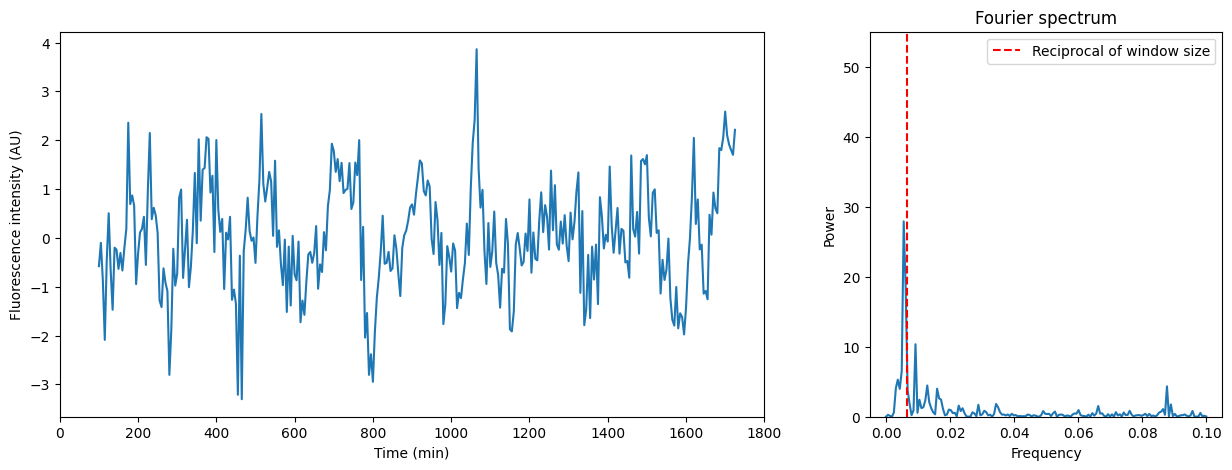
\includegraphics[width=\textwidth]{fft_slidingwindow}
   \caption{
   }
   \label{fig:analysis-slidingwindow-movavg}
  \end{subfigure}

  \begin{subfigure}[htpb]{0.8\textwidth}
   \centering
   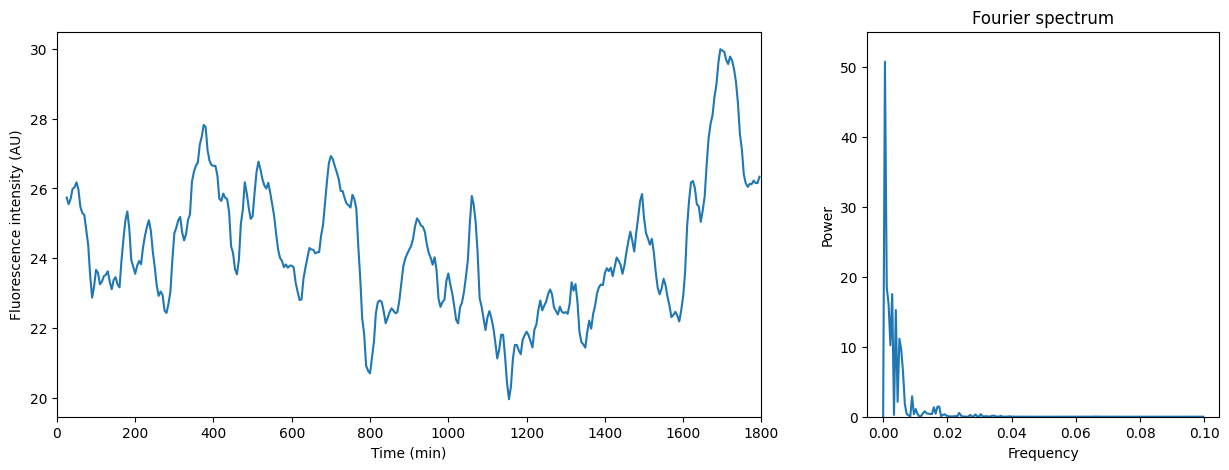
\includegraphics[width=\textwidth]{fft_savgol}
   \caption{
   }
   \label{fig:analysis-slidingwindow-savgol}
  \end{subfigure}

  \caption{
    (Left panels) Raw time series with trends, (middle panels) processed time series, and (right panels) Fourier spectra to demonstrate
    \textbf{(\ref{fig:analysis-slidingwindow-movavg})}
    using a moving average (window size 30), and
    \textbf{(\ref{fig:analysis-slidingwindow-savgol})}
    using a Savitzky-Golay filter (window size 7, polynomial order 3)
    to remove trends.
  }
  \label{fig:analysis-slidingwindow}
\end{figure}

Another caveat of this classifier lies in its sole tuning parameter, the false discovery rate, which affects the proportion of time series classed as oscillating.
To optimise the false discovery rate, labels of whether a time series is oscillatory were needed; if the labels are human-defined, as was the case in this section, any optimised false discovery rate would have low reliability.
Alternatively, a more reliable ground truth could be provided by an experiment expected to result in time series that are not oscillatory.
